\chapter{Using semantic distance to test the ortholog conjecture}

\section{Introduction}

The publication of the first high-throughput analysis of the ortholog conjecture using Gene Ontology (GO) received strong reactions from the biology community \citep{Thomas2012,Altenhoff2012,\Chen2012}.  While some objections, such as the assertion that overturning the conjecture would invalidate all comparative genomics, amount to \emph{paralogisms}, or illogical arguments; other objections warrant being addressed.  One such objection was that using the Maryland Bridge coefficient to compare annotations doe not properly account for annotation biases in GO data \citep{Altenhoff2012}.

\section{Results}

\subsection{Unfiltered, unnormalized results}

 We compared $S_{2}$ with ``excess schlicker" as implemented by \citet{Altenhoff2012} for molecular function annotations only.  
 
 
% \begin{figure*}[t!]
 
\begin{centering}

	\begin{subfigure}[b]{0.45\textwidth}
                \centering
                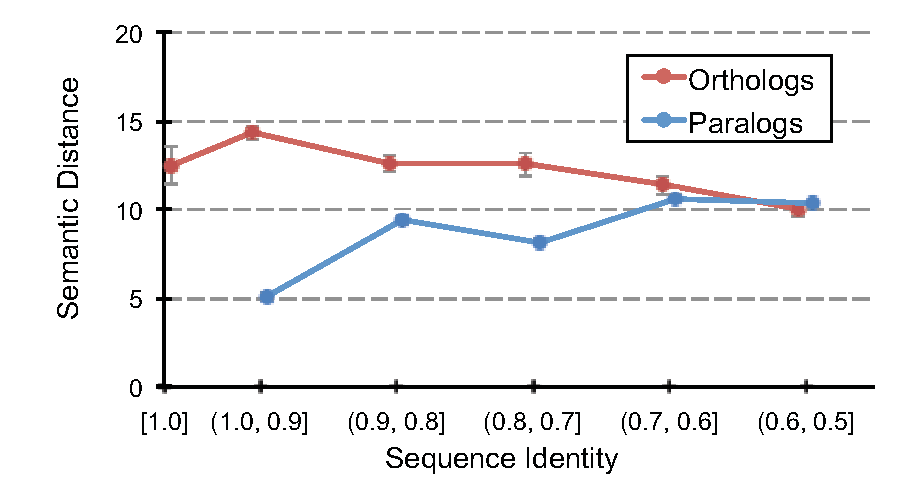
\includegraphics[width=\textwidth]{Figures/retesting/mfo_semantic_distance_unfiltered_2}
                \caption{$S_{2}$}
                \label{fig:unfilteredsd2}
        \end{subfigure}%
        \quad
	\begin{subfigure}[b]{0.45\textwidth}
                \centering
                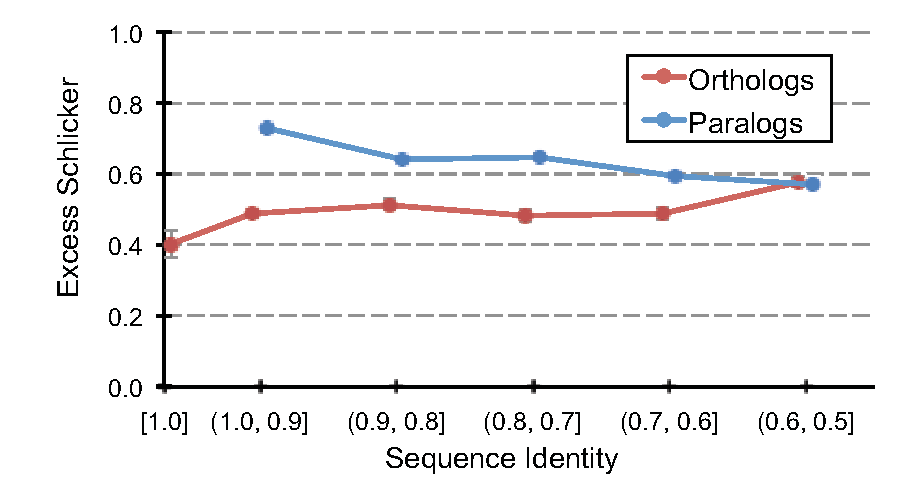
\includegraphics[width=\textwidth]{Figures/retesting/mfo_lin_unfiltered_2}
                \caption{Excess Schlicker}
                \label{fig:unfilteredlin2}
        \end{subfigure}
        
        	\begin{subfigure}[b]{0.45\textwidth}
                \centering
                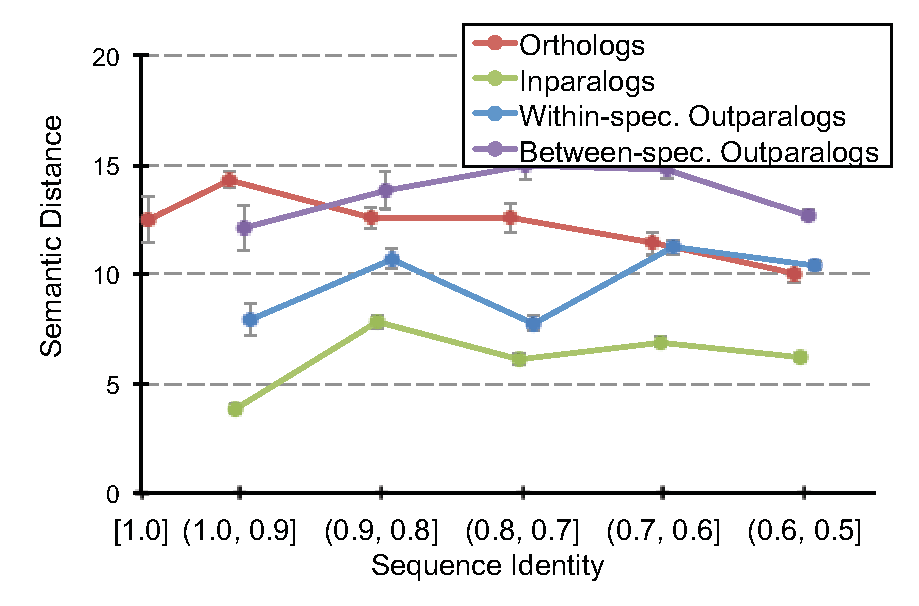
\includegraphics[width=\textwidth]{Figures/retesting/mfo_semantic_distance_unfiltered_4}
                \caption{$S_{2}$}
                \label{fig:unfilteredsd4}
        \end{subfigure}%
        \quad
	\begin{subfigure}[b]{0.45\textwidth}
                \centering
                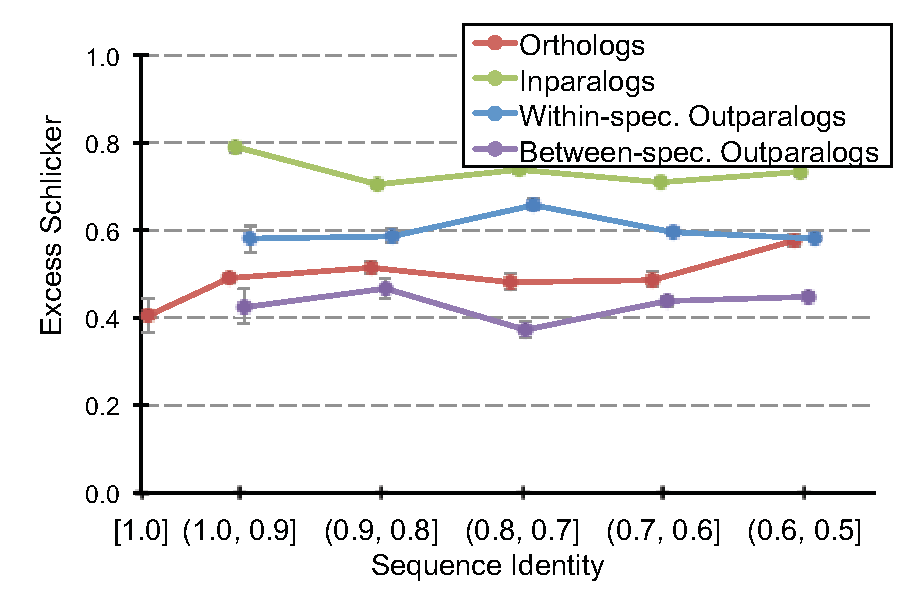
\includegraphics[width=\textwidth]{Figures/retesting/mfo_lin_unfiltered_4}
                \caption{Excess Schlicker}
                \label{fig:unfilteredlin4}
        \end{subfigure}

\end{centering}
\caption[Comparison of $S_{2}$ and ``Excess Schlicker"]{Comparison of $S_{2}$ and ``Excess Schlicker" for experimental molecular function annotations.  Results are not filtered for for common authorship, nor are they normalized based on the background similarity for each homology type and pair of organisms compared.}
\label{fig:unfiltered}
\end{figure*}



\subsection{Background normalized results}

We normalized 

%\input{Figures/retesting/unfiltered_normalized} 

 \subsection{Filtering based on common publication}

 
 \subsection{Comparison between $S_{2}$ and ``Excess Schlicker"}
 
  
  \subsection{The effect of normalization}
  
  \subsection{The effect of filtering annotations based on shared authorship}

%%%%%%%%%%%%%%%%%%%%%%
%%%%%%%%%%%%%%%%%%%%%%
\section{Methods}
%%%%%%%%%%%%%%%%%%%%%%
%%%%%%%%%%%%%%%%%%%%%%




%%%%%%%%%%%%%%%%%%%%%%
%%%%%%%%%%%%%%%%%%%%%%
%\subsection{Accounting for organism specific bias}
%%%%%%%%%%%%%%%%%%%%%%
%%%%%%%%%%%%%%%%%%%%%%

We previously defined improved methods for the evaluation of  GO annotations  (\Cref{sec:rumiMethods}). These metrics take into account dependencies between terms in the ontology and the discordance between the depth of a term in the ontology and its information content.  They can also easily be modified to account for organism specific biases in GO annotations by considering the information content of a term in a species specific manner.  For a given organism we calculate the organism specific information content, $i_{organism}(t)$, and accretion of a term, $ia_{organism}(t)$, using only proteins from that organism.  Given annotation subgraphs for two proteins, $T_{1}$ and $T_{2}$, that might or might not be from the same organisms,  $a$ and $b$, we calculate the organism specific semantic distance between the two subgraphs as

\[
S^{org}_{2}(T_{1},T_{2})=\left( \left[ \underset{t\in T_{1} \setminus T_{2}}{\sum} ia_{a}(t) \right]^{2} + \left[ \underset{t\in T_{2} \setminus T_{1}}{\sum} ia_{b}(t) \right]^{2} \right)^{1/2}
\]

As done in \citet{Altenhoff2012} this allows for the information content of a term measured based on the organism from which a particular gene is drawn.

In order to compare our results to those obtained by \citet{Altenhoff2012} we also implemented what they refer to as ``Excess Schlicker" similarity.  In spite of the potentially misleading name, this metric is actually similar to that defined by \citet{Lin1998}, not \citet{Schlicker2006}.  They define ``Excess Schlicker" similarity as

\begin{equation}
s(t_{1},t_{2})=\frac{ i_{org1}( \mathcal{A}(t_{1},t_{2}) ) + i_{org2}( \mathcal{A}(t_{1},t_{2}) ) }{i_{org1}(t_{1})+i_{org2}(t_{2})},
\end{equation}

Note that, in this case we are utilizing the set of leaf terms associated with each protein $\mathcal{L}(T_{1})$ and $\mathcal{L}(T_{2})$, and are utilizing the max-averaging method of averaging similarity between multiple leaf terms to obtain a single similarity value between genes (\Cref{sec:averaging}).



%%%%%%%%%%%%%%%%%%%%%%
%%%%%%%%%%%%%%%%%%%%%%
\subsection{Calculating the background similarity for types of homologs}
%%%%%%%%%%%%%%%%%%%%%%
%%%%%%%%%%%%%%%%%%%%%%

We also calculated the background similarity for each type of homolog for each pair of organisms compared.  This consisted of creating a pool of sequences from a given organism that had at least one relationship of the type being considered (1:1 orthologs, other orthologs, between-species outparalogs, within-species outparalogs, and inparalogs). We then randomly sampled 10,000 pairs of sequences from the pool of sequences for each pair of organism and homology type. We ensured that, when calculating the background for homology types defined between pairs of genes from different organisms (1:1 orthologs, other orthologs, between-species outparalogs), only random pairs of genes from different organisms were used to calculate the background similarity.  Similarly, when calculating the background similarity for homology types defined for pairs of genes from the same organisms (inparalogs and within-species outparalogs), we ensured that random pairs of genes did not consist of comparisons between a gene and itself.

If for a particular homology type and pair of organisms, or when calculating the background similarity within an orgasm, there were fewer than 2 sequences in the pool we did not calculate the background similarity and that species homology type was not included in the final normalized results.  This was done because the background similarity would closely mimic the actual distribution of similarity due to the small sample size.

\subsection{Accounting for publication bias}

In order to account for disparity in the number of paralogs annotated by the same pauthor (confirm this) we filtered annotations for pairs of genes that had PUBMED IDS (REF) associated with the same author name.  this was done in two ways.  In the first we removed both annotations associated with the same author. In the second we only removed one.  Because this method leads to ambiguity regarding which annotation should be excluded we randomly shuffled the list of annotations 20 times for each homolog pair; removing the annotation highest in the list.  We avoided cases where filtering annotations based on authorship could not be randomized.  These were cases where one way to exclude annotations due to one or both protein's having only one annotation that shares authorship with the other sequence.  One example of this is XXX and YYY.


